\subsection{\nue appearance in long baseline experiments and the quest for \dcp}
As mentioned in~\ref{sec:theta13}, the main goal of long baseline experiments is nowadays the search for \nue and \nueb appearance. The \nue appearance is in fact a sub-leading effect of the disappearance of muon neutrinos depending on a combination of \thint, \thatm, \dcp, and mass hierarchy as shown in Eq.~\ref{eq:theta13app}.

The \nue appearance phenomenon has been observed for the first time by T2K in 2012~\cite{Abe:2013hdq}. A total of 28 electron neutrino candidates were detected in Super-Kamiokande while $4.92\pm0.55$ background events were expected for $\thint=0$. The \ptheta distribution for these events is shown in Fig~\ref{fig:t2kapp} and the significance of this measurement correspond to 7.3\sigma. In 2016 also the NOVA experiment has reported the observation of \nue appearance.

By combining the observation of \nue apperance in long-baseline experiments with the precise measurement of \nueb disappearance with reactors it is possible to extract information on the sub-leading terms entering the appearance probability, particularly the CP violation term \dcp and the mass hierarchy sign. 
The relative size of the effect on the apperance probability due to \dcp and to the mass ordering depends on the baseline. The effect of the hierarchy is in fact proportional to the amount of matter crossed by neutrinos before reaching the detector. 

In the case of T2K the baseline is relatively short (295 km) and the matter effects contribute to $\sim\pm10\%$ of the oscillation probability while the effect due to \dcp can be as large as $\pm30\%$ for the extreme values of \dcp as shown in Fig.~\ref{fig:t2kappprob}. In the case of NOVA the baseline is 810 km and the effect of the mass ordering and of \dcp on \papp is roughly equal and it corresponds to $\sim20\%$ for each source.

\begin{figure} [h!]
\begin{center}
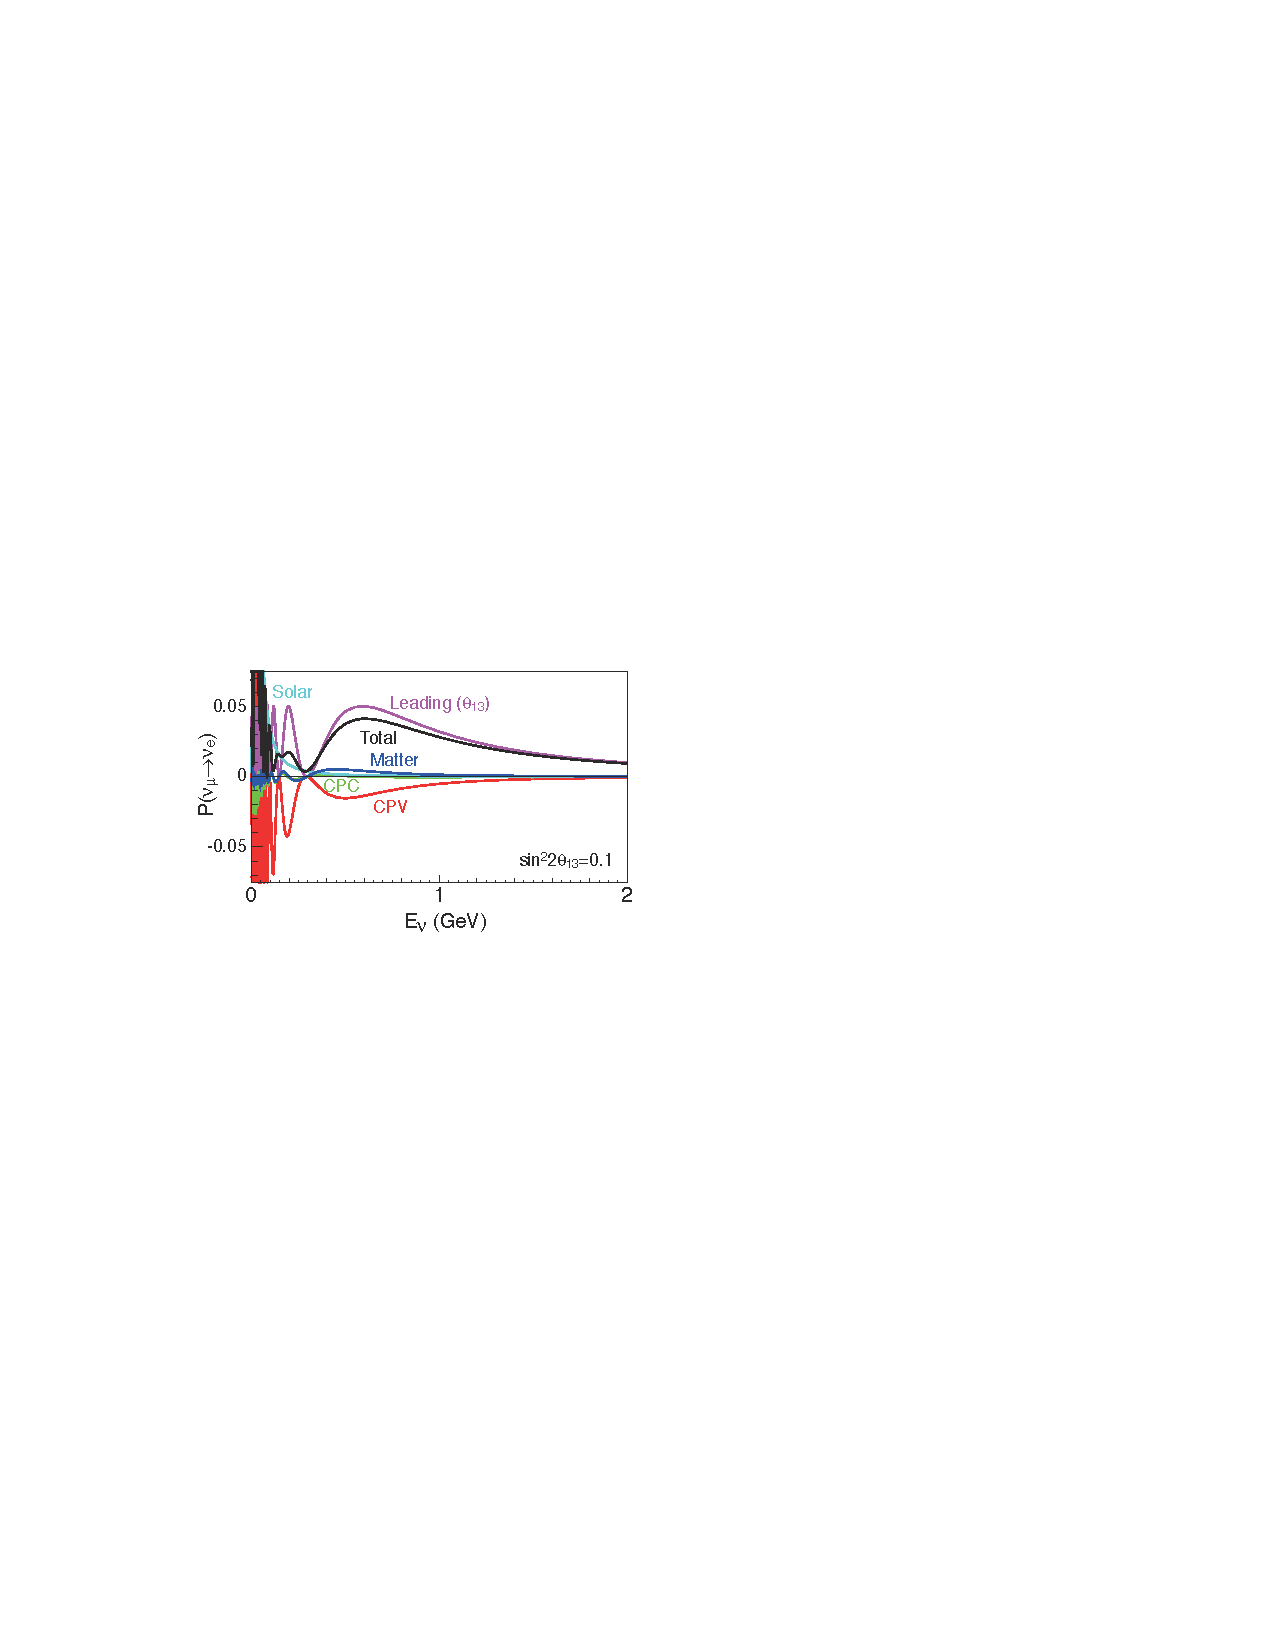
\includegraphics[width=8cm]{plotPhysics/papp_prob_2.pdf}
\caption{\label{fig:t2kappprob} Oscillation probabilities as a function of neutrino energy with L=295 km, \stot = 0.1, \dcp=$\pi/2$ and normal hierarchy. The contribution of the different terms of the oscillation probability is shown separately.}
\end{center}
\end{figure}

It is important to notice that for \nueb appearance the signs are reverted. In neutrino mode the appearance probability is maximized for normal hierarchy and $\dcp=-\pi/2$ while in anti-neutrino mode the appearance probability is maximized for inverted hierarchy and $\dcp=\pi/2$ as it is shown in Fig.~\ref{fig:t2kappnub} for the case of T2K. This figure clearly show the complementarity between \papp and \pappb and illustrates the importance of taking data also focusing anti-neutrino to fully exploit the asymmetry between \nue and \nueb apperance to measure \dcp.

\begin{figure} [h!]
\begin{center}
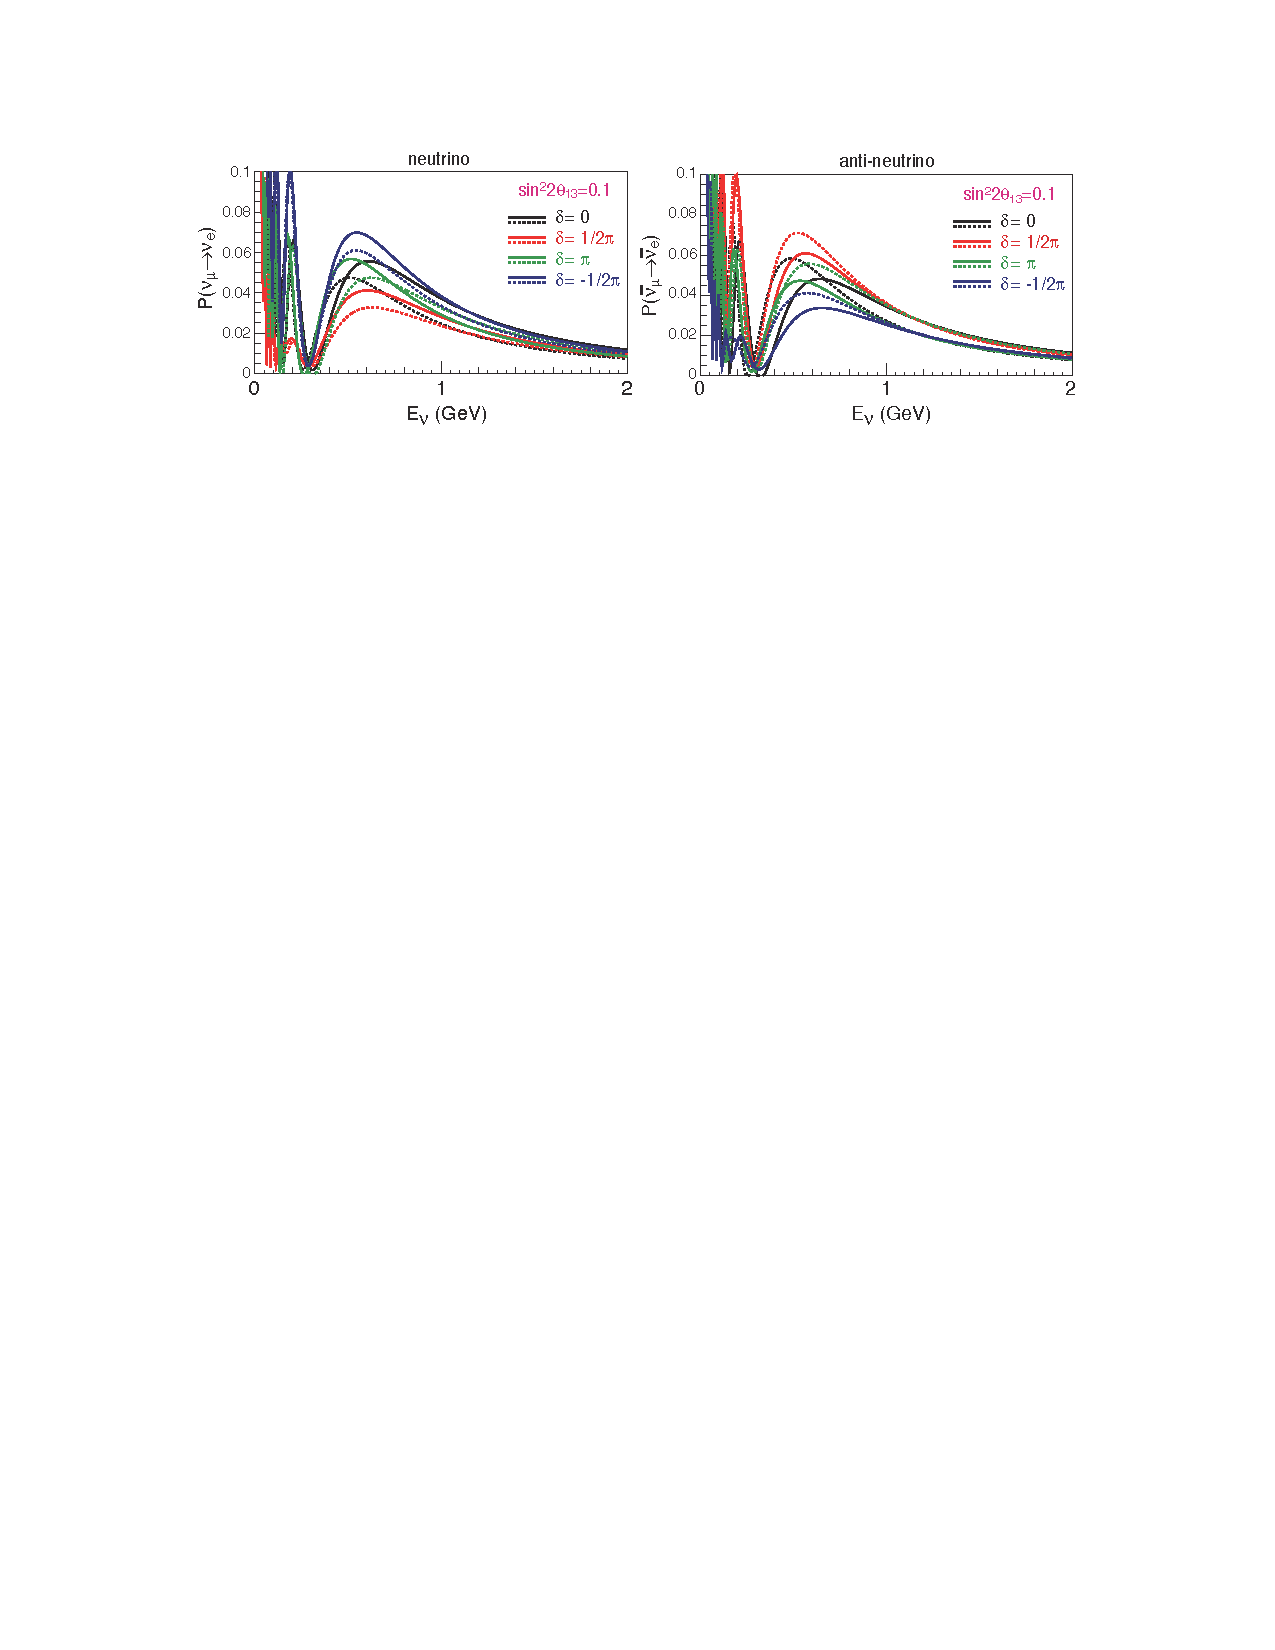
\includegraphics[width=14cm]{plotPhysics/papp_prob.pdf}
\caption{\label{fig:t2kappnub} Oscillation probabilities as a function of neutrino energy for \papp (left) and \pappb (right) with L=295 km and \stot = 0.1. The different line colors correspond to different values of \dcp while the solid (dashed) lines represent the normal (inverted) hierarchy.   }
\end{center}
\end{figure}

Finally Eq.~\ref{eq:theta13app} shows that the appearance probability also depends on the value of \thatm. Long-baseline accelerator experiments searching for \nue appearance are also sensitive to \thatm through \num disappearance.To fully take into account the correlations between oscillation parameters it is preferable to perform a joint analysis of appearance and disappearance as illustrated in~\cite{ 
 

\subsubsection{ \nue appearance in long baseline experiments}


T2K and NOVA (effect coupled to MH, NOVA if they publish)

nue appearance senstivity to delta CP (plot)


\subsubsection{ Search for \dcp in Super-Kamiokande}
SK effect in atm due to delta